\section{Algoritmo discreto de retroproyección filtrada}

La retroproyección filtrada discreta implementa la fórmula continua de FBP mediante operaciones finitas en la variable del detector y una cuadratura angular. En esta sección se separan la retroproyección sin filtrar, el filtrado por columnas y la reconstrucción final.

\subsection*{Retroproyección discreta}

El operador continuo de retroproyección está dado por
\[
\mathcal R^*g(x)=\int_0^\pi g(x\cdot\omega(\theta),\theta)\,d\theta,
\]
con $\omega(\theta)=(\cos\theta,\sin\theta)$. En la malla discreta se aproxima por
\[
(\mathcal R_d^*g)_{i,j}
=
\Delta\theta\sum_{k=0}^{M-1}
\mathcal I_t\bigl[g_{\cdot,k}\bigr]
\bigl(t(x_i,y_j,\theta_k)\bigr),
\]
donde $\mathcal I_t$ denota interpolación lineal en la variable del detector. La geometría matemática usa $t(x,y,\theta)=x\cdot\omega(\theta)$; en la implementación matricial se toma en cuenta la orientación vertical de las filas para evaluar correctamente las coordenadas cartesianas.

La retroproyección sin filtrar se obtiene aplicando directamente este operador al sinograma:
\[
f_{\mathrm{BP}}=\mathcal R_d^*g.
\]
Como se discutió en el capítulo anterior, $\mathcal R^*\mathcal R$ no es la identidad; por ello esta reconstrucción presenta difuminado y requiere filtrado previo.

\subsection*{Filtrado discreto por columnas}

El filtrado se aplica independientemente a cada columna angular $g_{\cdot,k}\in\mathbb R^{N_t}$. Para distinguir la transformada de Fourier continua de la transformada discreta usada en el código, se introducen los siguientes operadores:
\begin{itemize}
    \item $P:\mathbb R^{N_t}\to\mathbb R^{N_{\mathrm{fft}}}$, operador de zero-padding centrado.
    \item $C:\mathbb R^{N_{\mathrm{fft}}}\to\mathbb R^{N_t}$, operador de recorte al intervalo detector original.
    \item $F_{N_{\mathrm{fft}}}$, DFT de longitud $N_{\mathrm{fft}}$.
    \item $M_\tau[m]=\tau(\sigma_m)$, vector multiplicador evaluado en la grilla de frecuencias $\sigma_m$ generada con \texttt{fftfreq}.
\end{itemize}

Para cada columna angular se calcula
\[
g^\tau_{\cdot,k}
=
C F_{N_{\mathrm{fft}}}^{-1}
\operatorname{diag}(M_\tau)
F_{N_{\mathrm{fft}}}
P g_{\cdot,k}.
\]
En los experimentos se usa
\[
N_t=256,
\qquad
N_{\mathrm{fft}}=1024.
\]
La longitud $N_{\mathrm{fft}}$ es auxiliar: no añade datos ni resolución espacial. Su función es reducir los efectos de tratar directamente cada proyección finita como si fuera periódica, es decir, mitigar artefactos asociados a la convolución circular de la DFT.

\subsection*{Reconstrucción filtrada}

Luego de filtrar todas las columnas, la reconstrucción se define como
\[
f_\tau=\mathcal R_d^*g^\tau.
\]
Para la rampa canónica,
\[
\tau_{\mathrm{rampa}}(\sigma)=|\sigma|,
\]
esta expresión es la contraparte discreta de
\[
f=\mathcal R^*\mathcal F_t^{-1}\bigl[|\sigma|\,\mathcal F_t(\mathcal Rf)\bigr].
\]
No se introducen factores $1/2$, $1/\pi$, correcciones empíricas ni reescalamientos de las reconstrucciones.

La Figura~\ref{fig:chapter3-bp-vs-fbp} compara la retroproyección sin filtrar con la reconstrucción FBP usando la rampa.

\begin{figure}[htbp]
    \centering
    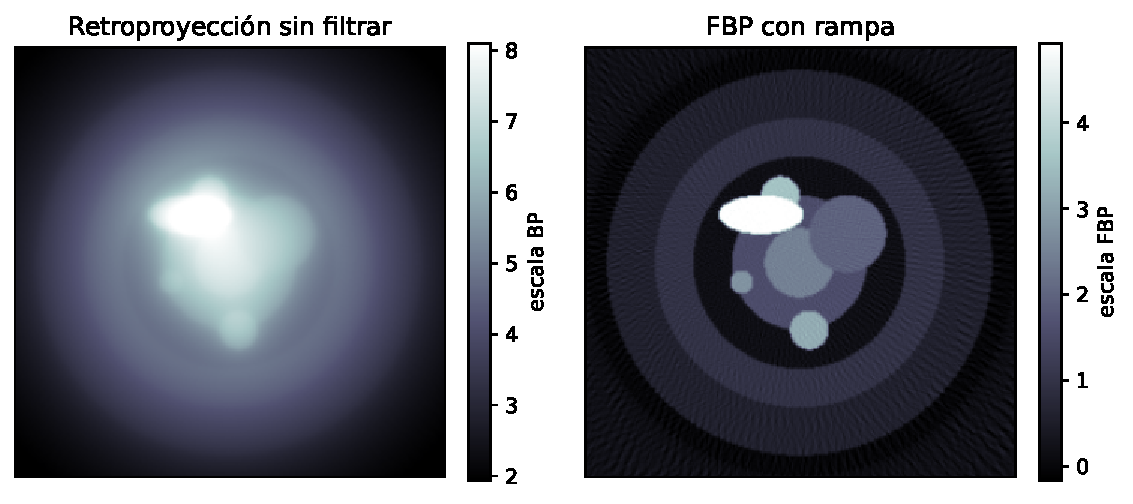
\includegraphics[width=0.86\textwidth]{Figures/Chapter3/bp_vs_fbp.pdf}
    \caption{Comparación entre la retroproyección sin filtrar y la retroproyección filtrada con la rampa. La retroproyección directa produce una imagen difuminada, mientras que el filtrado previo compensa parcialmente el suavizado asociado a $\mathcal R^*\mathcal R$.}
    \label{fig:chapter3-bp-vs-fbp}
\end{figure}
